\documentclass{beamer}
\usepackage[utf8]{inputenc}
\usepackage[brazil]{babel}
\usetheme{Malmoe}

\title[Universidade Católica do Salvador]{Extração de Informações de Dependência entre Módulos de Programas C/C++}
\author[Joenio Costa]{Joenio Marques da Costa}
\institute{UCSal - Universidade Católica do Salvador}
\date{junho de 2009}
\subject{alguma coisa}
\logo{
\includegraphics[scale=0.15]{imagens/brasao-ucsal-pb}}

\begin{document}

\frame{\titlepage} %para criar a página de rosto

\begin{frame}
 \tableofcontents
\end{frame}

\section{Introdução}

\begin{frame}
\frametitle{Introdução}
  \begin{itemize}
  \item<1-> O que é arquitetura de software.
  \item<1-> Porque documentar arquitetura de software.
  \item<1-> Como documentar arquitetura de software.
  \end{itemize}
\end{frame}

\section{Conceitos}

\begin{frame}
\frametitle{Conceitos}
  \begin{itemize}
  \item<1-> Coesão.
  \item<1-> Acoplamento.
  \item<1-> Atributos de modularidade.
  \end{itemize}
\end{frame}

\subsection{Coesão}

\begin{frame}
\frametitle{Coesão}
\framesubtitle{definição}
Coesão é a medida que define o quanto um módulo de um programa está focado em
solucionar um único problema. Quanto maior a coesão menor o acoplamento
\end{frame}

\subsection{Acoplamento}

\begin{frame}
\frametitle{Acoplamento}
\framesubtitle{definição}
Acoplamento representa o nível de interdependências entre os módulos de um
sistema. Quanto maior o acoplamento maior a complexidade.
\end{frame}

\section{Implementação do Extrator}

\begin{frame}
\frametitle{Implementação do Extrator}
 O extrator foi implementado como uma extensão para o
 egypt\footnote{http://www.gson.org/egypt} utilizando o
 Doxygen\footnote{http://www.doxygen.org} como base.
\end{frame}

\subsection{egypt}

\begin{frame}
\frametitle{egypt}
\framesubtitle{o que é}
 O egypt é um Software Livre desenvolvido com o objetivo de gerar grafos de
 chamada entre funções de programas escritos em C/C++.
\end{frame}

\begin{frame}
\frametitle{egypt}
\framesubtitle{como funciona}
 \begin{figure}[h]
 \center
 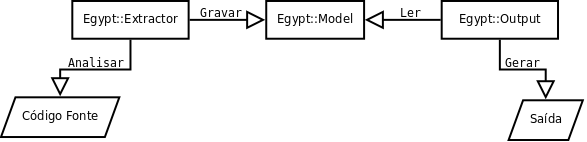
\includegraphics[scale=0.3]{imagens/egypt-fluxogram}
 \label{fig:egypt-fluxogram}
 \end{figure}
\end{frame}

\subsection{Doxygen}

\begin{frame}
\frametitle{Doxygen}
\framesubtitle{o que é}
 Doxygen é um sistema de documentação para C++, C, Java, Objective-C, Python,
 IDL, Fortran, VHDL, PHP e C\#.
\end{frame}

\begin{frame}
\frametitle{Doxygen}
\framesubtitle{o que pode fazer}
 O Doxygen possui um parser para cada linguagem suportada, assim ele consegue extrair
 informações de hierarquia e colaboração entre os módulos do projeto.
\end{frame}

\begin{frame}
\frametitle{Doxygen}
\framesubtitle{como funciona}
 \begin{figure}[h]
 \center
 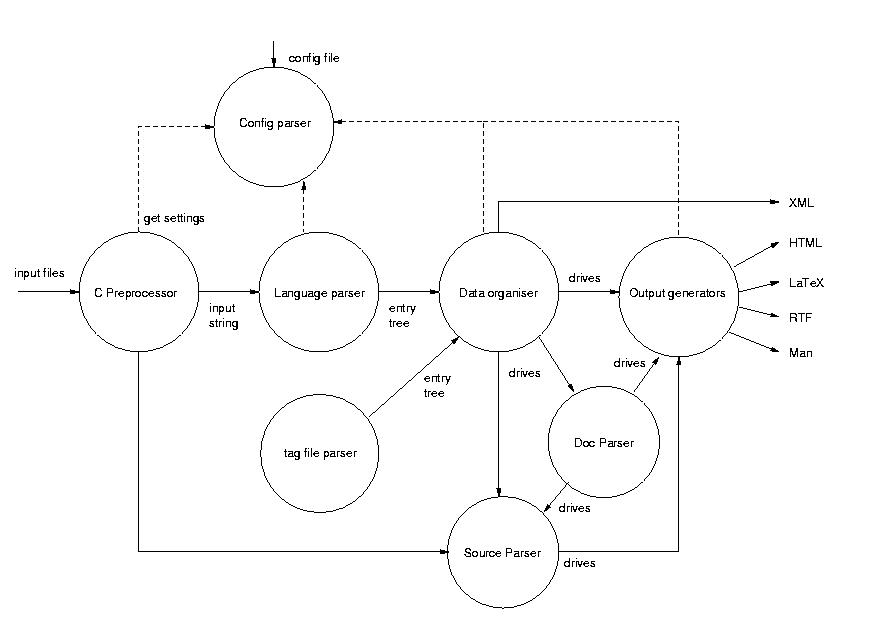
\includegraphics[scale=0.25]{imagens/doxygen-internals-flow}
 \label{fig:doxygen-internals-flow}
 \end{figure}
\end{frame}

\subsection{Implementação do Extrator}

\begin{frame}
\frametitle{Implementação do Extrator}
\framesubtitle{doxyparse\footnote{http://gitorious.org/projects/doxygen}}
 Um parser capaz de analisar projetos escritos em C/C++ e identificar onde os
 símbolos são declarados e utilizados dentro do do projeto.
 \begin{figure}[h]
 \center
 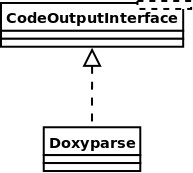
\includegraphics[scale=0.3]{imagens/doxyparse-diagram}
 \label{doxyparse-diagram}
 \end{figure}
\end{frame}

\begin{frame}
\frametitle{Implementação do Extrator}
\framesubtitle{egypt + doxyparse}
 Doxygen é um sistema de documentação para C++, C, Java, Objective-C, Python,
 IDL, Fortran, VHDL, PHP e C\#.

http://github.com/terceiro/egypt/
\end{frame}

\section{Avaliação}

\begin{frame}
\frametitle{Avaliação}
 conteúdo do slide
\end{frame}

\subsection{Procedimento}

\begin{frame}
\frametitle{Avaliação}
\framesubtitle{Procedimento}
 conteúdo do slide
\end{frame}

\subsection{Resultados}

\begin{frame}
\frametitle{Avaliação}
\framesubtitle{Resultados}
 conteúdo do slide
\end{frame}

\section{Conclusão}

\begin{frame}
\frametitle{Conclusão}
 conteúdo do slide
\end{frame}

\subsection{Trabalhos futuros}

\begin{frame}
\frametitle{Conclusão}
\framesubtitle{Trabalhos futuros}
 conteúdo do slide\cite{measuringCouplingAndCohesion}
\end{frame}

\section{}

\begin{frame}
\frametitle{Referências}
\bibliographystyle{abbrv}
\bibliography{bibliografia}{}
\end{frame}
\end{document}
